\section{Zipper Examples}

%%%% begin [list] %%%%
\begin{frame}[fragile, allowframebreaks]
\frametitle{Context for List}

\begin{itemize}
\item \lstinline.datatype 'a list = Nil | Cons 'a ('a list).

\item How to define a ``pointer'' \lstinline|p| into a list \lstinline|l|, supporting:
\begin{itemize}
	\item \lstinline|p = begin(l)|
	\item \lstinline|p->prev|
	\item \lstinline|p->next|
	\item \lstinline|*p := a|
\end{itemize}
\end{itemize}

\framebreak

\begin{itemize}
\newcommand{\AL}[1]{\textcolor{red}{#1}}
\newcommand{\AM}[1]{\textcolor[RGB]{0,170,0}{#1}}
\newcommand{\AR}[1]{\textcolor{blue}{#1}}
\item
\begin{lstlisting}
'a list_pointer = <@\AL{'a list} * \AM{'a} * \AR{'a list}@>
\end{lstlisting}
\begin{itemize}
	\item
\begin{lstlisting}
<@(\AL{... <- x <- x}) (\AM{y}) (\AR{z -> z -> ...})@>
\end{lstlisting}
\end{itemize}

\item \lstinline.begin (Cons x xs) = (Nil, x, xs).

\item \lstinline.prev (x#xs, y, zs) = (xs, x, y#zs).
\begin{itemize}
	\item
\begin{lstlisting}
<@(\AL{... <- x}) (\AL{x}) (\AM{y} -> \AR{z -> z -> ...})@>
\end{lstlisting}
\end{itemize}

\item \lstinline.next (xs, y, z#zs) = (y#xs, z, zs).
\begin{itemize}
	\item
\begin{lstlisting}
<@(\AL{... <- x <- x} <- \AM{y}) (\AR{z}) (\AR{z -> ...})@>
\end{lstlisting}
\end{itemize}

\item \lstinline.assign (xs, _, zs) y = (xs, y, zs).

\item \lstinline.reconstruct (xs, y, zs) = rev xs @ [y] @ zs.

\item Equivalent definition:
\begin{itemize}
	\item \lstinline.'a list_pointer = 'a * 'a list_context.
	\item \lstinline.'a list_context = 'a list * 'a list.
\end{itemize}
\end{itemize}
\end{frame}
%%%% end [list] %%%%

%%%% begin [btree] %%%%
\begin{frame}[fragile]
\frametitle{Context for Binary Tree I}

\newcommand{\AX}[1]{\textcolor{red}{#1}}
\newcommand{\AC}[1]{\textcolor{blue}{#1}}
\newcommand{\AL}[1]{\textcolor[RGB]{0,170,0}{#1}}
\newcommand{\AR}[1]{\textcolor{cyan}{#1}}
\newcommand{\AT}[1]{\textcolor{gray}{#1}}

\begin{itemize}
\item \lstinline.'a btree = Leaf | Node 'a ('a btree) ('a btree).

\item
\begin{lstlisting}
'a btree_pointer = <@\AX{'a}@> * 'a btree_context
\end{lstlisting}

\item
\begin{lstlisting}
'a btree_context = <@\AC{'a btree * 'a btree}@>
                   * 'a btree_ancestors
\end{lstlisting}

\item
\begin{lstlisting}
'a btree_ancestors =
    <@\AT{Top}@>
  | <@\AL{IsLeft}@>  'a ('a btree) ('a btree_ancestors)
  | <@\AR{IsRight}@> 'a ('a btree) ('a btree_ancestors)
\end{lstlisting}

\begin{itemize}
\item
\begin{lstlisting}
(<@\AX{2}, \AC{Leaf, Leaf}@>,
 <@\AR{IsRight 1 Leaf} (\AL{IsLeft 0 (Node 3 Leaf Leaf)} \AT{Top})@>)
\end{lstlisting}

\begin{onlyenv}<+>
\begin{lstlisting}
(Node 0 (Node 1 Leaf
                (Node <@\AX{2}@> Leaf
                        Leaf))
        (Node 3 Leaf
                Leaf))
\end{lstlisting}
\end{onlyenv}

\begin{onlyenv}<+>
\begin{lstlisting}
(Node 0 (Node 1 Leaf
                (Node 2 <@\AC{Leaf}@>
                        <@\AC{Leaf}@>))
        (Node 3 Leaf
                Leaf))
\end{lstlisting}
\end{onlyenv}

\begin{onlyenv}<+>
\begin{lstlisting}
(Node 0 (Node <@\AR{1 Leaf}@>
                (Node 2 Leaf
                        Leaf))
        (Node 3 Leaf
                Leaf))
\end{lstlisting}
\end{onlyenv}

\begin{onlyenv}<+>
\begin{lstlisting}
(Node <@\AL{0}@> (Node 1 Leaf
                (Node 2 Leaf
                        Leaf))
        <@\AL{(Node 3 Leaf}@>
                <@\AL{Leaf)}@>)
\end{lstlisting}
\end{onlyenv}

\begin{onlyenv}<+>
\color{gray}
\begin{lstlisting}
(Node 0 (Node 1 Leaf
                (Node 2 Leaf
                        Leaf))
        (Node 3 Leaf
                Leaf))
\end{lstlisting}
\end{onlyenv}
\end{itemize}

\end{itemize}
\end{frame}
%%%% end [btree] %%%%

%%%% begin [tree 2] %%%%
\begin{frame}[fragile]
\frametitle{Context for Binary Tree II}

\newcommand{\AX}[1]{\textcolor{red}{#1}}
\newcommand{\AC}[1]{\textcolor{blue}{#1}}
\newcommand{\AL}[1]{\textcolor[RGB]{0,170,0}{#1}}
\newcommand{\AR}[1]{\textcolor{cyan}{#1}}
\newcommand{\AT}[1]{\textcolor{gray}{#1}}

\begin{itemize}
\item \lstinline|up, down, left, right| for \lstinline|btree_pointer|:

\item
\begin{lstlisting}
  up (<@\AX{a}@>, (<@\AC{lc, rc}@>, <@\AL{IsLeft}@> p r anc))
   = (<@\AX{p}@>, (<@\AC{Node a lc rc, r}@>, anc))
| up (<@\AX{a}@>, (<@\AC{lc, rc}@>, <@\AR{IsRight}@> p l anc))
   = (<@\AX{p}@>, (<@\AC{l, Node a lc rc}@>, anc))
\end{lstlisting}

\item
\begin{lstlisting}
  left (<@\AX{a}@>, (<@\AC{llc, lrc}@>, <@\AR{IsRight}@> p (Node b rlc rrc) anc))
     = (<@\AX{b}@>, (<@\AC{rlc, rrc}@>, <@\AL{IsLeft}@>  p (Node a llc lrc) anc))
\end{lstlisting}

\item \lstinline|down| and \lstinline|right| are defined similarly

\item Simpler definition:\\
\begin{lstlisting}
'a btree_pointer = <@\AX{'a}@> * 'a bree_context
'a btree_context = <@\AC{'a btree * 'a btree}@>
                 * (<@\AL{bo}\AR{ol}@> * 'a * 'a btree) list
\end{lstlisting}
\end{itemize}
\end{frame}
%%%% end [btree 2] %%%%

%%%% begin [tree] %%%%
\begin{frame}[fragile, allowframebreaks]
\frametitle{Context for Ordered Tree}

\begin{itemize}
\item
\begin{lstlisting}
'a tree = Leaf | Node 'a ('a tree list)
\end{lstlisting}

\item
\begin{lstlisting}
'a tree_pointer = 'a * 'a tree_context
\end{lstlisting}

\item 
\begin{lstlisting}
'a tree_context = 'a tree list * 'a tree_ancestors
\end{lstlisting}

\item 
\begin{lstlisting}
'a tree_ancestors =
    Top
  | IsChild ('a tree list) 'a ('a tree list)
            ('a tree_ancestors)
\end{lstlisting}

\item \lstinline|up, down left, right| for \lstinline|tree_pointer|
\begin{itemize}
\item  similar with the ones for \lstinline|btree_pointer|
\end{itemize}

\item 
Simpler definition:\\
\begin{lstlisting}
'a tree_context = 'a tree list
           * ('a tree list * 'a * 'a tree list) list
\end{lstlisting}
\end{itemize}

\framebreak

Zipper!\footnote[frame]{Image source: www.pacifictrimming.com}

\begin{columns}
\begin{column}{0.75\textwidth}
\begin{figure}
\centering
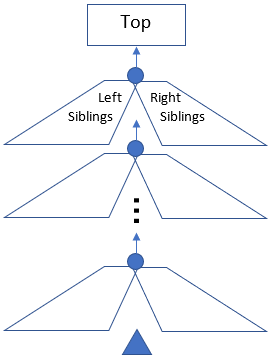
\includegraphics[width=0.6\textwidth]{figure/zipper}
\end{figure}
\end{column}
\begin{column}{0.3\textwidth}
\begin{figure}

\includegraphics[width=0.7\textwidth]{figure/real_zipper}
\end{figure}
\end{column}
\end{columns}

\end{frame}
%%%% end [tree] %%%%

%%%% begin [tree] %%%%
\begin{frame}[fragile]
\frametitle{Huet's Zipper}

\newcommand{\AS}[1]{\textcolor{red}{#1}}
\newcommand{\AL}[1]{\textcolor{blue}{#1}}

\begin{itemize}
\item For ordered trees with \AL{payload only on leaves}:

\begin{itemize}
\item
\begin{lstlisting}
'a ltree = <@\AL{Leaf 'a}@> | Node <@\AL{\st{'a}}@> ('a ltree list)
\end{lstlisting}
\end{itemize}

\item Focus on a \AS{subtree} instead of an element

\begin{itemize}
\item
\begin{lstlisting}
'a ltree_pointer = <@\AS{\st{'a} \underline{'a ltree}}@> * 'a ltree_context
\end{lstlisting}

\item 
\begin{lstlisting}
'a ltree_context = <@\AS{\st{'a ltree list *}}@> 'a ltree_ancestors
\end{lstlisting}

\item 
\begin{lstlisting}
'a ltree_ancestors =
    Top
  | IsChild ('a ltree list) <@\AL{\st{'a}}@> ('a ltree list)
            ('a ltree_ancestors)
\end{lstlisting}

\end{itemize} 

\end{itemize}
\end{frame}

